\chapter{Discussion}
Please tell more about conclusion and how to the next work of this study.

\section{Andri Fajar Sunandhar / 1164065}
\subsection{Teori}
\begin{enumerate}
\item Mengapa file suara harus dilakukan MFCC, dilengkapi dengan ilustrasi atau gambar.
\par Mel Frequency Cepstral Coefficients (MFCC) merupakan koefisien yang merepresentasikan audio. Sehingga diharuskannya melakukan MFCC kepada objek suara atau audio agar suara dapat berubah atau diubah ke dalam bentuk data matrix dimana telah dilakukan ekstraksi oleh MFCC kemudian direalisasikan sebagai data matrix. Ilustrasinya bisa dilihat pada gambar berikut  \ref{no1}.
	\begin{figure}[ht]
	\centerline{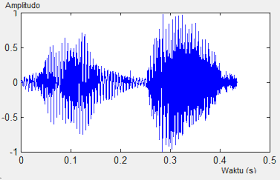
\includegraphics[width=0.5\textwidth]{figures/chapter6/no1.png}}
	\caption{Gambar MFCC.}
	\label{no1}
	\end{figure}

\item Konsep dasar Neural Network, dilengkapi dengan ilustrasi atau gambar.
\par Neural Network merupakan kategori ilmu Soft Computing. Neural Network sebenarnya mengadopsi dari kemampuan otak manusia yang mampu memberikan stimulasi/rangsangan, melakukan proses, dan memberikan output. Output diperoleh dari variasi stimulasi dan proses yang terjadi di dalam otak manusia. Kemampuan manusia dalam memproses informasi merupakan hasil kompleksitas proses di dalam otak. Misalnya, yang terjadi pada anak-anak, mereka mampu belajar untuk melakukan pengenalan meskipun mereka tidak mengetahui algoritma apa yang digunakan.  Ilustrasinya bisa dilihat pada gambar berikut   \ref{no2}.
	\begin{figure}[ht]
	\centerline{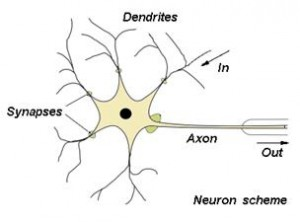
\includegraphics[width=0.5\textwidth]{figures/chapter6/no2.jpg}}
	\caption{Gambar Neural Network.}
	\label{no2}
	\end{figure}

\item Konsep pembobotan Neural Network, dilengkapi dengan ilustrasi atau gambar.
\par Sebuah Neural Network dikonfigurasi untuk aplikasi tertentu, seperti pengenalan pola atau klasifikasi data. Terjadi penglibatan dalam penyesuaian koneksi sinaptik yang ada antara neuron ketika melakukan penyempurnaan dengan proses pembelajaran. Penyesuaian nilai bobot yang ada pada tiap konektivitas baik dari input, neuron maupun output disinkronkan dengan penyesuaian koneksi sinaptik antar neuron itu sendiri.  Ilustrasinya bisa dilihat pada gambar berikut  \ref{no3}.
	\begin{figure}[ht]
	\centerline{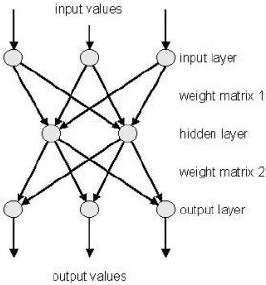
\includegraphics[width=0.5\textwidth]{figures/chapter6/no3.jpg}}
	\caption{Gambari Pembobotan neural network.}
	\label{no3}
	\end{figure}

\item Konsep fungsi aktifasi dalam Neural Network, dilengkapi dengan ilustrasi atau gambar
\par Operasi matematik yang dikenakan pada sinyal output y. Sehingga fungsi ini akan digunakan untuk pengaktifan dan juga penonaktifan neuron. Ilustrasinya bisa dilihat pada gambar berikut  \ref{no4}.
	\begin{figure}[ht]
	\centerline{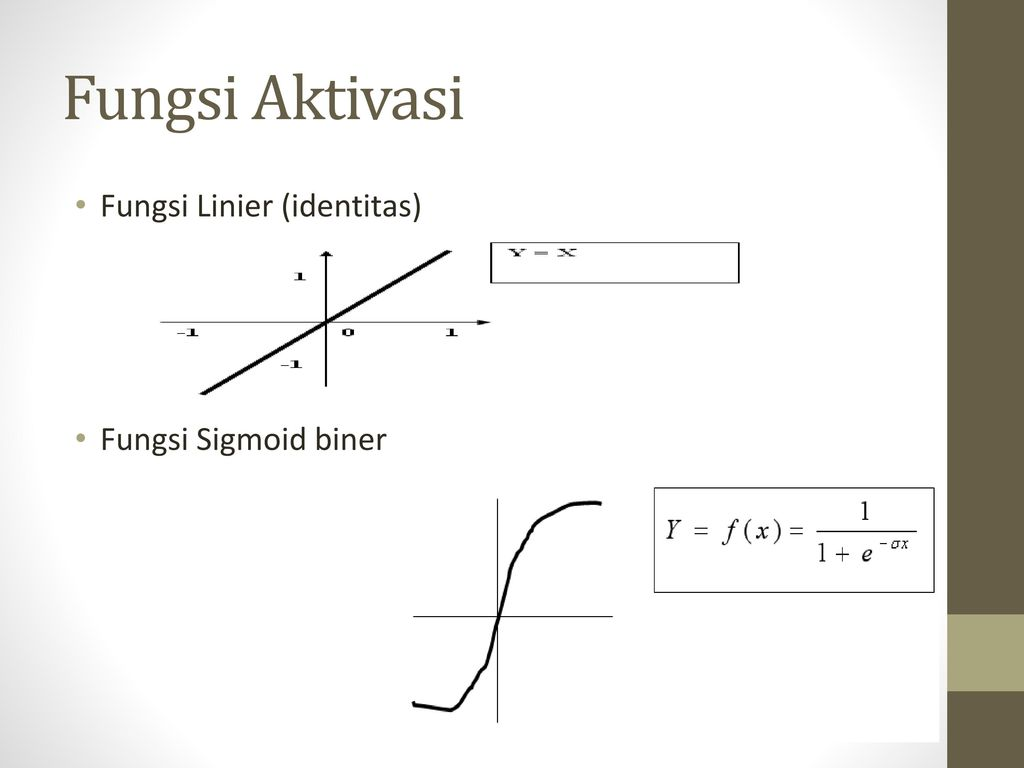
\includegraphics[width=0.5\textwidth]{figures/chapter6/no4.jpg}}
	\caption{Gambar Aktivitas neural network.}
	\label{no4}
	\end{figure}

\item Cara membaca hasil plot dari MFCC, dilengkapi dengan ilustrasi atau gambar.
\par Nanti akan ada outputan berbentuk grafik. Ada 3 dimensi atau sumbu. Dimana untuk sumbu x merupakan waktu, sedangkan sumbu y merupakan frekuensi dari suara yang dihasilkan dalam bentu Hz. Sedangkan pada bagian tengah atau sumbu z merupakan power atau kekuatan dari lagu atau suara atau desibel yang dihasilkan. Untuk melihat penjelasan dari warna pada gambar yang di tengah, maka kita harus mendownload gambar nya terlebih dahuhulu. Untuk warna biru itu merupakan suara rendah, yang merah merupakan tinggi dan daya frekuensi nya berada pada nilai yang rendah karena bass bekerja pada suara yang rendah. Tidak selalu tergantung pada warna untuk menentukan nilai atau frekuensinya. Tetapi pada jenis lagu yang dugunakan.  Ilustrasinya bisa dilihat pada gambar berikut \ref{no5m}
	\begin{figure}[ht]
	\centerline{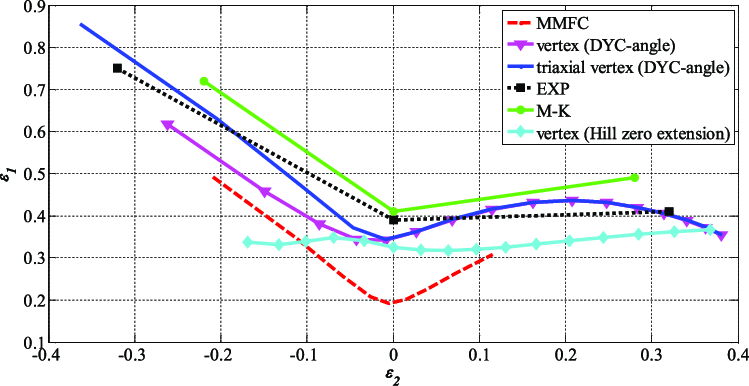
\includegraphics[width=0.5\textwidth]{figures/chapter6/no5.png}}
	\caption{Gambar Plot dari MFCC.}
	\label{no5m}
	\end{figure}

\item Apa itu One-Hot Encoding, dilengkapi dengan ilustrasi atau gambar.
\par One-Hot Encoding adalah sekelompok bit yang kombinasi hukumnya hanya terdiri dari bit dengan bit tinggi (1) dan bit lainnya rendah (0). Implementasi serupa di mana semua bit '1' kecuali satu '0' kadang-kadang disebut one-cold. Dalam statistik, variabel dummy mewakili teknik serupa untuk mewakili data kategorikal.  Ilustrasinya bisa dilihat pada gambar berikut  \ref{no6}.
	\begin{figure}[ht]
	\centerline{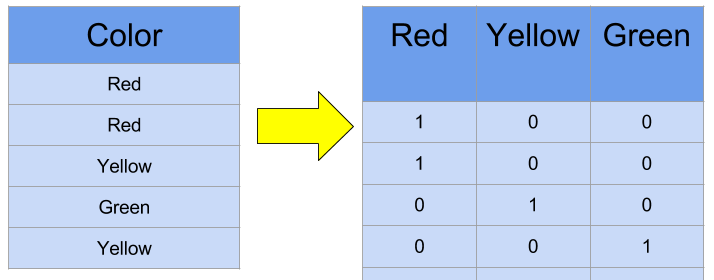
\includegraphics[width=0.5\textwidth]{figures/chapter6/no6.png}}
	\caption{Gambar One-hot Encoding.}
	\label{no6}
	\end{figure}

\item Fungsi dari np.unique dan to.categorical, dilengkapi dengan ilustrasi atau gambar.
\par Np.unique Berfungsi untuk menemukan elemen unik array.  Ilustrasinya bisa dilihat pada gambar berikut  \ref{no7a}.
Ada tiga output opsional selain elemen unik:
	\begin{itemize}
	\item Indeks array input yang memberikan nilai unik
	\item Indeks array unik yang merekonstruksi array input
	\item Berapa kali setiap nilai unik muncul dalam array input
	\end{itemize}
		\begin{figure}[ht]
		\centerline{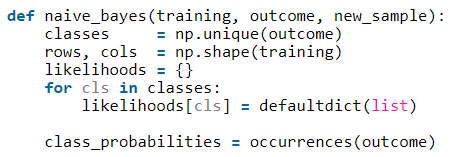
\includegraphics[width=0.5\textwidth]{figures/chapter6/no7a.png}}
		\caption{Gambar np.unique.}
		\label{no7a}
		\end{figure}

\par To.categorical Berfungsi untuk menemukan elemen unik array.  Ilustrasinya bisa dilihat pada gambar berikut  \ref{no7b}.
	\begin{figure}[ht]
	\centerline{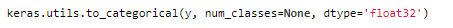
\includegraphics[width=0.5\textwidth]{figures/chapter6/no7b.png}}
	\caption{Gambar to.categorical.}
	\label{no7b}
	\end{figure}

\item Fungsi dari Sequential, dilengkapi dengan ilustrasi atau gambar.
\par Sebuah jenis model yang digunakan dalam perhitungan ataupun code program yang direalisasikan. Neural Networks Sequential membangun fitur tingkat tinggi melalui lapisannya yang berurutan. Sequential juga merupakan proses dimana membandingkan setiap elemen larik satu per satu secara beruntun, mulai dari elemen pertama, sampai dengan elemen terakhir atau elemen yang dicari sudah ditemukanl.  Ilustrasinya bisa dilihat pada gambar berikut  \ref{no8}.
	\begin{figure}[ht]
	\centerline{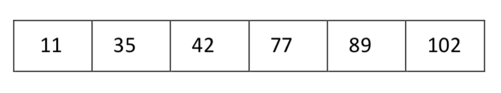
\includegraphics[width=0.5\textwidth]{figures/chapter6/no8.png}}
	\caption{Gambar Sequential.}
	\label{no8}
	\end{figure}
\end{enumerate}


\subsection{Praktek}
\begin{enumerate}
\item Data GTZAN Genre Collection dan data dari freesound. 
	\par Isi Data GTZAN Genre Collection adalah file musik yang difolderkan berdasarkan genre atau jenis lagu dan data freesound berisikan suara alam contohnya adalah suara lebah, suara air, dan sebagainya.
	\par Berikut adalah kode program untuk meload data tersebut :
	
	\par Berikut penjelasan dari kode program :
	\begin{itemize}
	\item membuat variabel untuk mendefinisikan direktori file yang akan digunakan.
	\item membuat variabel untuk meload atau memanggil variabel filename\_rock.
	\end{itemize}
	
	\par Apabila kode program dijalankan maka akan menghasilkan seperti gambar \ref{no9} :
		\begin{figure}[ht]
		\centerline{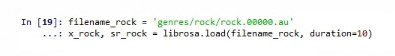
\includegraphics[width=0.5\textwidth]{figures/chapter6/no9.jpg}}
		\caption{Gambar Hasil Load.}
		\label{no9}
		\end{figure}

\item Fungsi dari display\_mfcc() .
	\par Berikut adalah kode program yang digunakan :
	
	\par Setelah kode program dijalankan, maka akan muncul seperti gambar \ref{10a} :
		\begin{figure}[ht]
		\centerline{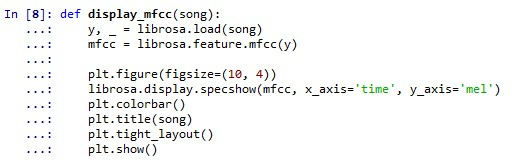
\includegraphics[width=0.5\textwidth]{figures/chapter6/no10a.jpg}}
		\caption{Gambar Display MFCC.}
		\label{no10a}
		\end{figure}
	\par Penjelasan Gambar :
	\begin{itemize}
	\item Baris 1 : membuat fungsi display mfcc untuk menampilkan vektorisasi dari sebuah suara
	\item Baris 2 : membuat variabel y untuk meload atau membaca variable song dari perintah librosa load song
	\item Baris 3 : membuat variabel mfcc untuk memenggil variabel y dan mengubah suara menjasi vektor
	\item Baris 4 : memploting gambar dengan ukuran 10x4
	\item Baris 5 : menampilkan spektogram/chromagram
	\item Baris 6 : menambahkan colorbar pada plot
	\item Baris 7 : menetapkan atau memberikan judul untuk suara
	\item Baris 8 : untuk memberikan label pada sumbu di grafik
	\item Baris 9 : fungsi untuk menampilkan hasil plot
	\end{itemize}
	\par Untuk menampilkan hasil ploting dilakukan perintah berikut :
	
	\par Apabila program tersebut dijalankan, maka akan muncul hasil seperti gambar \ref{no10} :
		\begin{figure}[ht]
		\centerline{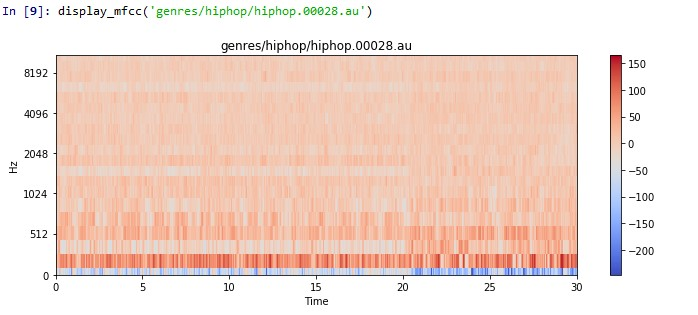
\includegraphics[width=0.5\textwidth]{figures/chapter6/no10.jpg}}
		\caption{Gambar hasil display.}
		\label{no10}
		\end{figure}
	\par Penjelasan kode : display MFCC digunakan untuk menampilkan hasil dari gambar \ref{no10a}. Dimana gambar tersebut menjelaskan kekuatan atau daya dari sebuah suara.

\item Fungsi dari extract\_features\_song().
	\par Untuk menggunakan fungsi dari extract\_features\_song() diimplementasikan pada kode berikut :
	
	\par Jika kode di atas dijalankan maka didapat hasil seperti gambar \ref{no11} :
		\begin{figure}[ht]
		\centerline{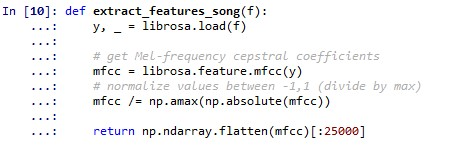
\includegraphics[width=0.5\textwidth]{figures/chapter6/no11.jpg}}
		\caption{Gambar extract feature.}
		\label{no11}
		\end{figure}
	\par Berikut adalah penjelasan dari gambar \ref{no11}:
	\begin{itemize}
	\item Baris 1 : membuat fungsi extract feature song dengan inputan f
	\item Baris 2 : membuat variabel y untuk meload atau membaca inputan f dari perintah librosa load song
	\item Baris 3 : membuat variabel mfcc untuk membuat feature dari variabel y
	\item Baris 4 : membuat normalisasi nilai antara -1 sampai 1
	\item Baris 5 : mengambil 25000 data pertama berdasarkan durasi suara atau musik lali dikembalikan salinan arraynya dan dikecilkan menjadi satu.
	\end{itemize}
	
	\par  Mengapa yang diambil 25.000 baris pertama? Karena menyesuaikan dengan kapasitas penyimpanan supaya tidak lemot.

\item Penjelasan kode program generate\_features\_and\_labels()
	\par Disini akan mengilustrasikan fungsi dari generate\_feature\_and\_labels(). Kode program yang digunakan adalah  seperti berikut :
	
	\par Apabila kode program tersebut dijalankan akan menghasilkan seperti pada gambar \ref{no12}.
		\begin{figure}[ht]
		\centerline{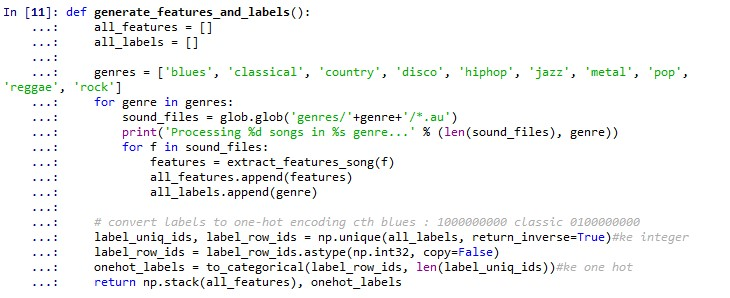
\includegraphics[width=0.5\textwidth]{figures/chapter6/no12.jpg}}
		\caption{Gambar Generate feture and label.}
		\label{no12}
		\end{figure}
	\par Berikut adalah penjelasan dari hasil gambar ilustrasi \ref{no12}:
	\begin{itemize}
	\item Baris 1 : membuat perintah fungsi generate features and labels
	\item Baris 2 : membuat variabel all features dengan array kosong
	\item Baris 3 : membuat variabel all labels dengan array kosong
	\item Baris 4 : Membuat variable yang berisi nama folder
	\item Baris 5 : membuat perintah fungsi looping
	\item Baris 6 : membuat atribut sound files yang berisi perintah looping perfolder dari folder genres dan mengambil semua file berekstensi au.
	\item Baris 7 : memunculkan berapa song.
	\item Baris 8 : membuat perintah fungsi
	\item Baris 9 : membuat variabel. features untuk memanggil fungsi extract features song (f) sebagai inputan. Setiap satu file array sound files dilakukan ekstrak fitur.
	\item Baris 10 : memasukkan semua features kedalam all features
	\item Baris 11 : memasukkan semua genres kedalam all labels
	\item Baris 12 : medefinisikan label uniq ids dan row ids untuk mengeksekusi perintah unix yang memiliki perameter atribut all labels dan return inverse.
	\item Baris 13 : Membuat variabel label\_row\_ids untuk menentukan type data 32 byte dari variabel tersebut.
	\item Baris 14 : Membuat variabel onehot\_labels yang akan mengeksekusi to\_categorical dengan variabel parameter low\_row\_ids dan len(label\_uniq\_ids)
	\item Baris 15 : Mengembalikan (return) dan menampilkan hasil eksekusi dari variabel parameter all\_features dan onehot\_labels perintah dari np.stack.
	\end{itemize}

\item penggunaan fungsi generate\_features\_and\_labels()
	\par Mengapa fungsi generate\_features\_and\_labels() sangat lama ketika meload dataset genre? Itu karena data yang diload sangat banyak sehingga membutuhkan waktu yang banyak
	\par Berikut kode program yang digunakan :
	
	\par Dari kode program tersebut dapat dijelaskan bahwa kode tersebut digunakan untuk passing parameter dari fitur ekstraksi menggunakan mfcc. Sehingga ketika dijalankan menghasilkan seperti gambar \ref{no13}.
		\begin{figure}[ht]
		\centerline{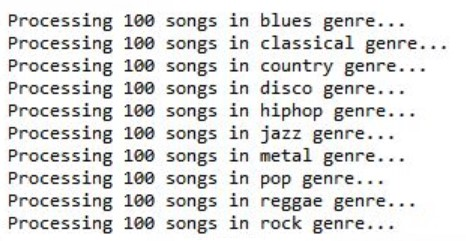
\includegraphics[width=0.5\textwidth]{figures/chapter6/no13.jpg}}
		\caption{Gambar Generate feture and label.}
		\label{no13}
		\end{figure}
	\par Gambar \ref{no13} menjelaskan setelah kode dieksekusi, program memproses 100 song setiap genre musik. Sehingga membutuhkan waktu yang lama.

\item Jelaskan kenapa harus dilakukan pemisahan data training dan data set sebesar 80 persen?
	\par Mengapa harus dilakukan pemisahan data training dan data testing dari dataset sebesar 80 persen, itu karena dataset yang digunakan akan dibuat klasifikasinya.
	\par Berikut adalah kode program yang digunakan :
	
	\par Penjelasan kode program :
	\begin{itemize}
	\item Membuat klasifikasi dengan plit data sebesar 80 persen data training dan 80 persen data testing.
	\end{itemize}
	
	\par Setelah kode program tersebut dijalankan, maka akan menghasilkan seperti gambar \ref{no14}:
	
		\begin{figure}[ht]
		\centerline{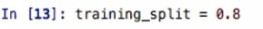
\includegraphics[width=0.5\textwidth]{figures/chapter6/no14.jpg}}
		\caption{Gambar hasil pemisahan.}
		\label{no14}
		\end{figure}

\item Fungsi Sequential()
	\par Kode program yang digunakan adalah sebagai berikut :
	
	\par Penjelasan parameter :
	\begin{itemize}
	\item sequential = merupakan sebuah model
	\item dense 100 = inputan awal neutron adalah 100.
	\item np.shape = mendapatkan bentuk array.
	\item relu = menjelaskan untuk inputan yang maksimum yang akan dipilih.
	\item dense 10 = outputan neutron adalah 10
	\item softmax = sebuah fungsi yang mengambil input vektor dari bilangan real K, dan menormalkannya menjadi distribusi probabilitas yang terdiri dari probabilitas K.
	\end{itemize}
	
	\par Setelah program dijalankan, maka akan menghasilkan seperti pada gambar \ref{no15}.
	
		\begin{figure}[ht]
		\centerline{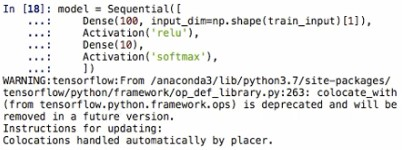
\includegraphics[width=0.5\textwidth]{figures/chapter6/no15.jpg}}
		\caption{Gambar Sequential.}
		\label{no15}
		\end{figure}
		
	\par Penjelasan gambar \ref{no15}:
	\begin{enumerate}
	\item Membuat model sequential
	\item Inputan awal neuton adaldah 100 yang diambil dari data train. 
	\item Melakukan aktivasi dengan parameter fungsi relu.
	\item Dense(10) merupakan outputan dari neural network  yang mengkategorikan 10 kategori jenis genre.
	\item Melakukan aktivasi dengan menggunakan parameter fungsi softmax.
	\end{enumerate}

\item Fungsi compile()
	\par Kode program yang digunakan adalah sebagai berikut :
	
	\par Penjelasan parameter :
	\begin{itemize}
	\item adam = algoritma optimisasi yang digunakan sebagai ganti dari prosedur penurunan gradien stokastik klasik untuk memperbarui bobot jaringan yang berulang berdasarkan data train.
	\item categorical\_crossentropy = parameter yang digunakan untuk menyusun sebuah model yang memiliki target dalam format kategorikal.
	\item accuracy = fungsi metrik yang digunakan untuk menilai kinerja model.
	\end{itemize}
	
	\par Setelah program dijalankan, maka akan menghasilkan seperti pada gambar \ref{no16}.
	
		\begin{figure}[ht]
		\centerline{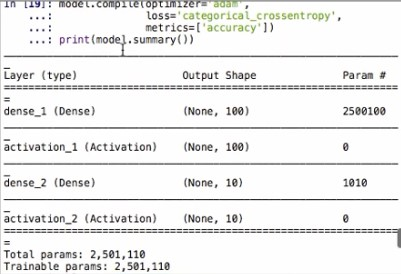
\includegraphics[width=0.5\textwidth]{figures/chapter6/no16.jpg}}
		\caption{Gambar hasil compilel.}
		\label{no16}
		\end{figure}
		
	\par Berikut adalah penjelasan gambar \ref{no16} :
	\begin{enumerate}
	\item Mengcompile model yang sudah dibuat. Dengan menggunakan algoritma optimisasi, fungsi loss, dan fungsi metrik.
	\item Lalu perintah print digunakan untuk menampilkan hasil yang berupa seperti tabel yang berisi tipe layer, dense, aktivasi, total params dan trainable param.
	\item Dense\_1 dan activation\_1 menunjukkan neuron inputan sebanyak 100.
	\item Dense\_2 dan activation\_2 menunjukkan neuron outputan sebanyak 10.
	\end{enumerate}

\item Fungsi fit()
	\par Kode program yang digunakan adalah sebagai berikut :
	
	\par Penjelasan parameter pada kode program :
	\begin{itemize}
	\item epochs = fungsi yang digunakan untuk menentukan berapa kali melakukan iterasi.
	\item batch\_size = fungsi yang digunakan untuk menentukan berapa file dalam satu epochs.
	\item validation\_split = melakukan pengecekan cross validasi.
	\end{itemize}
	
	\par Apabila kode program tersebut dijalankan, maka akan menghasilkan seperti pada gambar \ref{no17}.
	
		\begin{figure}[ht]
		\centerline{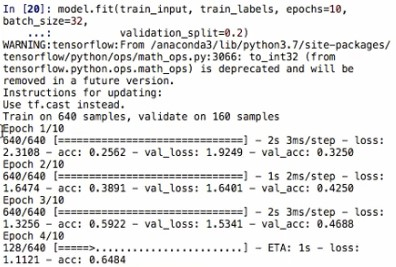
\includegraphics[width=0.5\textwidth]{figures/chapter6/no17.jpg}}
		\caption{Gambar fungsi fit.}
		\label{no17}
		\end{figure}
		
	\par Penjelasan hasil, perhatikan gambar \ref{no17} :
	\begin{enumerate}
	\item Melakukan pelatihan model dengan menggunakan perintah fit.
	\item Data yang digunakan adalah data training.
	\item Kemudian data training dilakukan iterasi atau dijalankan sebanyak 10 kali.
	\item Dan dalam satu epochs diberlakukan 32 file.
	\item Lalu diambil 20 persen data untuk dilakukan pengecekan cross validation.
	\end{enumerate}
	
	\par Dari gambar \ref{no17} kita dapat melihat bahwa setiap satu epoch terdapat nilai akurasi dan loss.

\item Fungsi evaluate()
	\par Berikut adalah kode program yang digunakan :
	
	\par Parameter yang digunakan pada kode program :
	\begin{itemize}
	\item  batch\_size = fungsi yang digunakan untuk menentukan berapa file yang digunakan.
	\end{itemize}
	
	\par Apabila kode program tersebut dijalankan, maka akan menghasilkan seperti pada gambar \ref{no18}.
	
		\begin{figure}[ht]
		\centerline{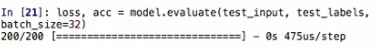
\includegraphics[width=0.5\textwidth]{figures/chapter6/no18.jpg}}
		\caption{Gambar fungsi evaluate.}
		\label{no18}
		\end{figure}
		
	\par Penjelasan hasil pada gambar \ref{no18} :
	\begin{enumerate}
	\item Membuat parameter loss dan acc untuk mengetahui dan mengevaluasi hasil prediksi data test, berapa kesalahannya dan berapa ketepatannya.
	\end{enumerate}

\item Fungsi predict()
	\par Berikut adalah kode program yang digunakan :
	
	\par Parameter yang digunakan pada kode program :
	\begin{itemize}
	\item [:1] = digunakan untuk menentukan batasa row.
	\end{itemize}
	
	\par Apabila kode program tersebut dijalankan, maka akan menghasilkan seperti pada gambar \ref{no19}.
	
		\begin{figure}[ht]
		\centerline{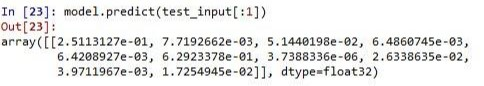
\includegraphics[width=0.5\textwidth]{figures/chapter6/no19.jpg}}
		\caption{Gambar fungsi predict.}
		\label{no19}
		\end{figure}
		
	\par Penjelasan hasil pada gambar \ref{no19} :
	\begin{enumerate}
	\item Mengetes hasil prediksi model dari data test\_input dengan batasan 1 row atau lagu nomor satu. Dan hasilnya berupa array dengan tipedata float32.
	\item Cara bacanya adalah 25 persen dari satu lagu tersebut bergenre blues, 77 persen bergenre classical, dan begitu pula seterusnya.
	\item Sehingga ditemukan paling tinggi dari lagu tersebut sebesar 64.8 persen yang bergenre disco.
	\end{enumerate}
\end{enumerate}

\subsection{Penanganan Error}
Dari praktek pemrograman yang dilakukan di modul ini, error yang kita dapatkan(hasil komputer sendiri) di dokumentasikan dan di selesaikan(nilai 5 per error yang ditangani. Untuk hari kedua):

\begin{enumerate}
	\item skrinsut error
		\begin{enumerate}
		\item Error :
			\begin{figure}[ht]
			\centerline{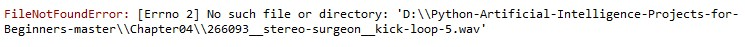
\includegraphics[width=0.5\textwidth]{figures/chapter6/error.jpg}}
			\caption{Gambar Sequential.}
			\label{error}
			\end{figure}
		\end{enumerate}
		
	\item Tuliskan kode error dan jenis errornya
		\begin{enumerate}
		\item Kode Error  :
			\begin{itemize}
				\item Kode error : FileNotFoundError: [Errno 2] No such file or directory: 'D: Python Artificial-Intelligence-Projects-for-Beginners-master  Chapter04 266093 stereo-surgeon kick-loop-5.wav'
				\item Jenis error : File Not FoundError
			\end{itemize}
		\end{enumerate}

	\item Solusi pemecahan masalah error
		\par Error yang terjadi pada gambar \ref{error} akibat dari kesalahan pada pengalamatan direktori sehingga file yang akan digunakan tidak ditemukan, oleh karena itu pengalamatan direktori disesuaikan dengan kebutuhan penggunaan.
	
		
\end{enumerate}
